\documentclass[a4paper,12pt,final]{memoir}

% misc
\renewcommand{\familydefault}{bch}	% font
\pagestyle{empty}					% no pagenumbering
\setlength{\parindent}{0pt}			% no paragraph indentation


% required packages (add your own)
\usepackage{flowfram}										% column layout
\usepackage[top=1cm,left=1cm,right=1cm,bottom=1cm]{geometry}% margins
\usepackage{graphicx}										% figures
\usepackage{url}											% URLs
\usepackage[usenames,dvipsnames]{xcolor}					% color
\usepackage{multicol}										% columns env.
	\setlength{\multicolsep}{0pt}
\usepackage{paralist}										% compact lists
\usepackage{tikz}

%%%%%%%%%%%%%%%%%%%%%%%%%%%%%%%%%%%%%
% Create column layout
%%%%%%%%%%%%%%%%%%%%%%%%%%%%%%%%%%%%%
% define length commands
\setlength{\vcolumnsep}{\baselineskip}
\setlength{\columnsep}{\vcolumnsep}

% left frame
\newflowframe{0.2\textwidth}{\textheight}{0pt}{0pt}[left]
	\newlength{\LeftMainSep}
	\setlength{\LeftMainSep}{0.2\textwidth}
	\addtolength{\LeftMainSep}{1\columnsep}
 
% small static frame for the vertical line
\newstaticframe{1.5pt}{\textheight}{\LeftMainSep}{0pt}
 
% content of the static frame
\begin{staticcontents}{1}
\hfill
\tikz{%
	\draw[loosely dotted,color=RoyalBlue,line width=1.5pt,yshift=0]
	(0,0) -- (0,\textheight);}%
\hfill\mbox{}
\end{staticcontents}
 
% right frame
\addtolength{\LeftMainSep}{1.5pt}
\addtolength{\LeftMainSep}{1\columnsep}
\newflowframe{0.7\textwidth}{\textheight}{\LeftMainSep}{0pt}[main01]


%%%%%%%%%%%%%%%%%%%%%%%%%%%%%%%%%%%%%
% define macros (for convience)
%%%%%%%%%%%%%%%%%%%%%%%%%%%%%%%%%%%%%
\newcommand{\Sep}{\vspace{1.5em}}
\newcommand{\SmallSep}{\vspace{0.5em}}

\newenvironment{AboutMe}
	{\ignorespaces\textbf{\color{RoyalBlue} About me}}
	{\Sep\ignorespacesafterend}
	
\newcommand{\CVSection}[1]
	{\Large\textbf{#1}\par
	\SmallSep\normalsize\normalfont}

\newcommand{\CVItem}[1]
	{\textbf{\color{RoyalBlue} #1}}


%%%%%%%%%%%%%%%%%%%%%%%%%%%%%%%%%%%%%
% Begin document
%%%%%%%%%%%%%%%%%%%%%%%%%%%%%%%%%%%%%
\begin{document}

% Left frame
%%%%%%%%%%%%%%%%%%%%
%
% Upload your own photo using the files menu
\begin{figure}
	\hfill
	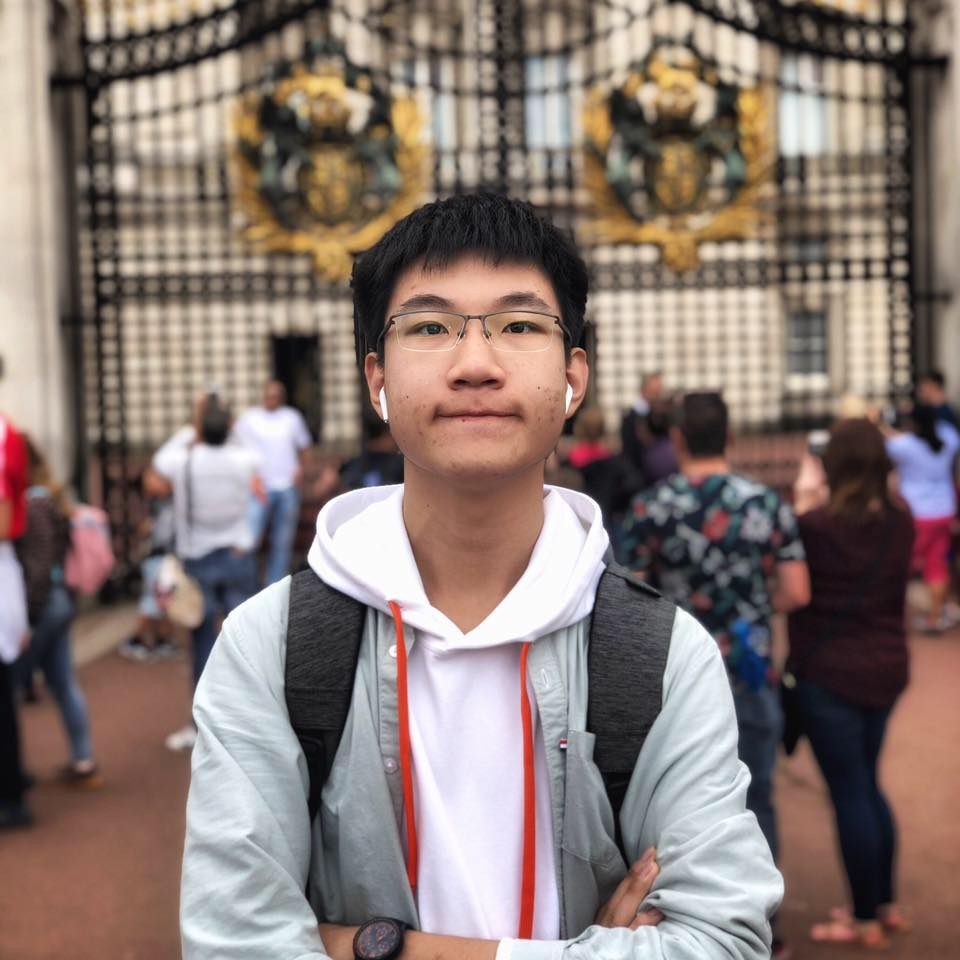
\includegraphics[width=0.8\columnwidth]{photo.jpg}
	\vspace{2cm}
\end{figure}

\begin{flushright}\small
	Chunxu LIU \\
	\url{181240035@smail.nju.edu.cn}  \\
	\url{lcxrocks.github.io/homepage/} \\
	+86-15022320541
\end{flushright}\normalsize
\framebreak


% Right frame
%%%%%%%%%%%%%%%%%%%%
\Huge\bfseries {\color{RoyalBlue} Chunxu LIU} \\
\Large\bfseries  Undergraduate in Computer Science Elite Program \\Nanjing University \\

\normalsize\normalfont

% About me
\begin{AboutMe}
	I was admitted to study in Kuang Yaming Honors School, Nanjing University in September 2018. After studying General Natural Sciences for one freshman semester, I declared Computer Science as my major. Through the training of my course in the previous two years, I have aquired the basic knowledge about computer science field and the ability to solve the problems independently. Since my learning of computer science begins, my passion towards it has never faded, so I would very much like to dive deeper into the area and keep studying.
\end{AboutMe}

% Experience
\CVSection{Experience}
\CVItem{May 1998 - Nov 2001, Lorem ipsum}\\
Lorem ipsum dolor sit amet, consectetur adipiscing elit. Vivamus vel bibendum metus. Proin rutrum pharetra molestie. Cras sollicitudin nulla nec leo lobortis in tristique purus pretium. Ut eu felis nulla.
\SmallSep

\CVItem{Jun 1995 - Apr 1998, Vivamus vel}\\
Lorem ipsum dolor sit amet, consectetur adipiscing elit. Vivamus vel bibendum metus.

\Sep

% Education
\CVSection{Education}
\CVItem{September 2018 - present, Elite Program of Computer Science}\\
BSc. Computer Science, Nanjing University
\SmallSep

\CVItem{July 2020 - August 2020, Machine Learning Plus Deep Learning Summer Online Program}\\
Massachusetts Institute of Technology \\ 
Finished in Nanjing University
\SmallSep

\CVItem{July 2019 - August 2019, Advanced Business and British Culture Summer Program}\\
Hertford College, Oxford University\\
Finished in Oxford University, Britain
\SmallSep

% You'll need these 3 lines at the end of each page!
% \clearpage
% \framebreak
% \framebreak

\CVItem{2005 - 2007, Vivamus vel bibendum}\\
Proin rutrum pharetra molestie. Cras sollicitudin nulla nec leo lobortis in tristique purus pretium. Ut eu felis nulla.
\Sep


% Skills
\CVSection{Skills}
\CVItem{Platforms}
% \begin{multicols}{3}
% \begin{compactitem}[\color{RoyalBlue}$\circ$]
% 	\item Lorem 
% 	\item Ipsum 
% \end{compactitem}
% \end{multicols}
\SmallSep

\CVItem{Computer software}
\begin{multicols}{3}
\begin{compactitem}[\color{RoyalBlue}$\circ$]
	\item Lorem 
	\item Ipsum 
	\item Dolor 
	\item Sit 
	\item Amet
	\item Consectetur 
	\item Adipiscing 
	\item Elit
	\item \ldots
\end{compactitem}
\end{multicols}
\Sep 

% References
% \CVSection{References}
% References upon request.

%%%%%%%%%%%%%%%%%%%%%%%%%%%%%%%%%%%%%
% End document
%%%%%%%%%%%%%%%%%%%%%%%%%%%%%%%%%%%%%
\end{document}